\section{Hasil dan Pembahasan}\label{sec:hasil}

Seluruh angka pada bagian ini berasal dari satu eksekusi penuh
\texttt{notebooks/pipeline.ipynb} dan disalin dari berkas \texttt{reports/fase2/*.csv}
yang dihasilkannya. Angka turunan (selisih, panen, korelasi) dihitung dari berkas yang
sama.

\subsection{Validitas Pipeline}\label{sec:validitas}

Pemeriksaan kewarasan lolos. Cabang teks QS-OCR mereproduksi CNN~1D Fase~1
\textbf{bit-identik} per seed (OA 0,7345 / 0,7248 / 0,7204, dengan epoch terbaik yang
sama), walaupun dilatih ulang dari nol dengan kode baru. Cabang citra mencapai
$0{,}8169 \pm 0{,}0257$, di dalam toleransi terhadap Fase~1 ($0{,}8086 \pm 0{,}0210$).
Seed 44 jelas lebih lemah (0,7808, epoch terbaik 11), sedangkan seed 42 dan 43 mencapai
0,8315 dan 0,8386.

\subsection{Analisis Data Eksploratif per Modalitas}\label{sec:eda}

Analisis ini dijalankan sebelum pelatihan apa pun, pada seluruh 3.482 dokumen. Analisis
yang memakai label (kata khas, \textit{probe}, jalan pintas kode ID) hanya dipasang pada
bagian latih seed 42, sedangkan data uji hanya dipakai untuk mengukur akurasi
\textit{probe}. Untuk teks, yang dianalisis di sini adalah kondisi acuan QS-OCR;
perbandingan antar-mesin ada pada Subbagian~\ref{sec:hasil-ocr}.

\subsubsection{Distribusi Kelas dan Pembagian Data}

Kelas Tobacco3482 timpang: Memo 620 dokumen, Email 599, Letter 567, Form 431, Report
265, Scientific 261, Advertisement 230, Note 201, News 188, dan Resume 120, sehingga rasio
kelas terbesar terhadap terkecil 5,17. Pembagian terstratifikasi menghasilkan 720 dokumen
latih, 80 validasi, dan 2.682 uji dengan komposisi kelas yang sama di ketiga seed. Resume
hanya punya 25 dokumen latih dan 3 dokumen validasi per seed, dan Note 41 dan 5.

\subsubsection{Modalitas Citra}

Citra JPG beresolusi tinggi. Lebar halaman berkisar 817 sampai 3.520 piksel dengan median
1.728 piksel. Bila halaman diasumsikan berukuran \textit{letter}, perkiraan resolusinya
96 sampai 414 dpi, median 203 dpi, dan kuartil atas 299 dpi. Statistik citra per kelas
ditunjukkan Gambar~\ref{fig:eda-citra}.

\begin{figure}[H]
  \centering
  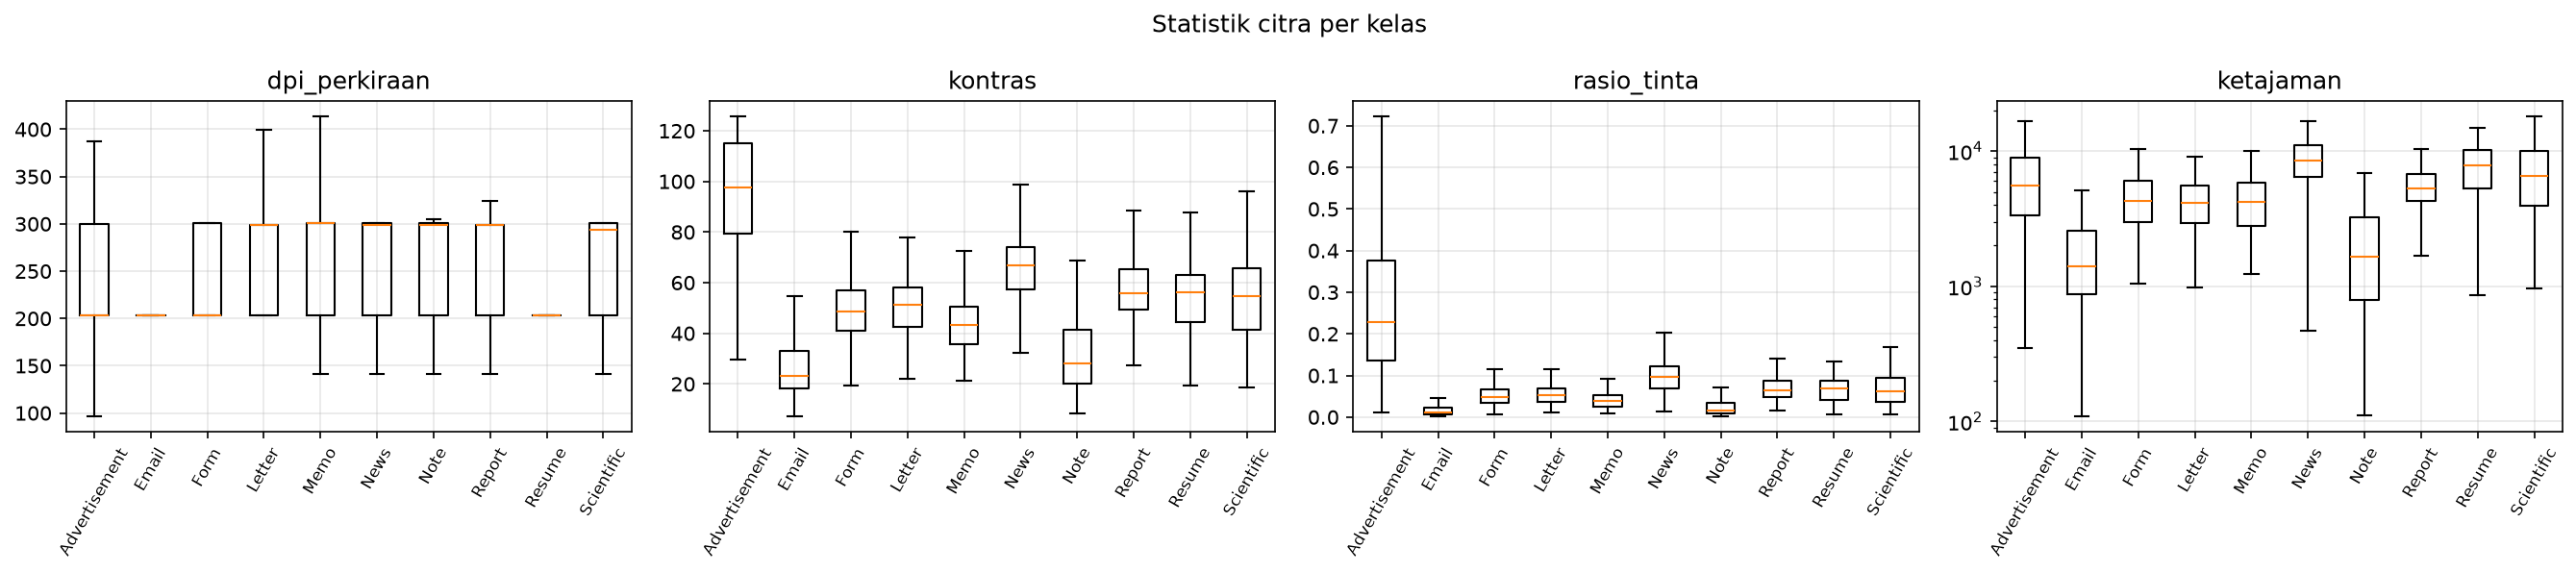
\includegraphics[width=\textwidth]{../../reports/figures/fase2_eda_statistik_citra.png}
  \caption{Statistik citra per kelas: perkiraan dpi, kontras, rasio tinta, dan ketajaman
  (variansi Laplacian, skala log)}
  \label{fig:eda-citra}
\end{figure}

Gambar~\ref{fig:eda-citra} memperlihatkan tiga hal.
\begin{enumerate}
  \item \textbf{Resolusi tidak seragam antar-kelas.} Seluruh halaman Email dan Resume
  berada di 203 dpi, sedangkan kelas lain menyebar antara 203 dan 300 dpi. Resolusi asli
  hilang setelah citra diubah ke $384\times384$, tetapi pola ini menunjukkan kelas-kelas
  itu dipindai dengan cara berbeda, sehingga menjadi sumber bias yang potensial.
  \item \textbf{Advertisement jauh lebih gelap.} Kontras dan rasio tintanya paling tinggi
  (median rasio tinta sekitar 0,23, kelas lain sekitar 0,1 atau kurang), karena halaman
  iklan didominasi gambar.
  \item \textbf{Email dan Note paling jarang tintanya}, sehingga ketajamannya juga paling
  rendah. Variansi Laplacian bergantung pada jumlah tepi, jadi halaman yang sedikit
  tulisannya otomatis mendapat skor rendah walaupun tidak kabur.
\end{enumerate}

\textit{Linear probe} (regresi logistik) di atas fitur MobileNetV2 ImageNet tanpa
\textit{fine-tune} mencapai \textbf{OA 0,7293} dan macro F1 0,7099, padahal menebak kelas
mayoritas hanya 0,1782. Tata letak halaman sudah sangat informatif bahkan tanpa pelatihan
khusus dokumen. Pada proyeksi t-SNE (Gambar~\ref{fig:eda-tsne}, kiri), Email,
Advertisement, Form, News, Resume, dan Scientific membentuk kelompok yang jelas, sedangkan
Letter, Memo, dan Report bercampur di tengah. Ketiganya adalah dokumen ketikan
berparagraf dengan tata letak yang mirip.

\subsubsection{Modalitas Teks}

Teks QS-OCR berpanjang median 174 kata per dokumen (rata-rata 224, maksimum 1.579).
Sebanyak 1,1\% dokumen tidak berisi satu pun kata, dan 7,8\% lebih panjang dari 500 kata
sehingga terpotong saat masuk CNN~1D. Laju OOV (Persamaan~\ref{eq:oov}) bermedian 5,5\%
dan rata-rata 9,8\%. Angka ini batas bawah galat OCR, dan tidak dapat dibandingkan dengan
$\pm$26\% yang dilaporkan \textcite{audebert2020}, yang memakai kamus lebih ketat.

Masalah teks terpusat di dua kelas (Tabel~\ref{tab:eda-penanda}). Ambang penanda diambil
dari ekor distribusi data (persentil 5 atau 95): teks pendek $\leq 23$ kata dan OOV tinggi
$\geq 0{,}369$.

\begin{table}[H]
  \centering
  \caption{Persentase dokumen bertanda masalah teks per kelas (QS-OCR)}
  \label{tab:eda-penanda}
  \fontsize{10}{12}\selectfont
  \begin{tabular}{|l|r|r|r|}
    \hline
    \textbf{Kelas} & \textbf{Teks kosong} & \textbf{Teks pendek} & \textbf{OOV tinggi} \\ \hline
    Note & 14,4\% & 41,3\% & 30,8\% \\ \hline
    Advertisement & 3,5\% & 17,4\% & 13,0\% \\ \hline
    Form & 0\% & 1,4\% & 10,7\% \\ \hline
    News & 0\% & 2,1\% & 8,0\% \\ \hline
    Kelas lain & 0\% & $\leq 4{,}2$\% & $\leq 3{,}4$\% \\ \hline
    \textbf{Semua} & 1,1\% & 4,7\% & 4,9\% \\ \hline
  \end{tabular}
\end{table}

Note berisi banyak tulisan tangan dan catatan pendek, sedangkan iklan sering berteks
sedikit atau dipindai terputar $90^\circ$, yang tidak dikenali Tesseract dengan
\texttt{-{}-psm 3}. Kata dengan bobot TF-IDF tertinggi per kelas
(Tabel~\ref{tab:eda-tfidf}) menunjukkan bahwa teks OCR tetap membawa penanda kelas yang
kuat. Kelas Note lagi-lagi berbeda: daftarnya berisi potongan kata rusak seperti
\texttt{ore} dan \texttt{ous}.

\begin{table}[H]
  \centering
  \caption{Kata TF-IDF tertinggi per kelas (bagian latih seed 42, QS-OCR)}
  \label{tab:eda-tfidf}
  \fontsize{10}{12}\selectfont
  \begin{tabularx}{\textwidth}{|l|>{\raggedright\arraybackslash}X|}
    \hline
    \textbf{Kelas} & \textbf{Kata khas} \\ \hline
    Advertisement & warning, surgeon, cigarette, general, advertisement, smoking, tar, nicotine \\ \hline
    Email & sent, subject, message, original, wednesday, date, thanks, meeting \\ \hline
    Form & date, fax, number, pages, form, total, morris \\ \hline
    Letter & tobacco, dear, research, new, sincerely, york \\ \hline
    Memo & correspondence, attached, philip, morris, memorandum \\ \hline
    News & said, smoking, health, smoke, tobacco, smokers \\ \hline
    Note & desk, information, james, ore, web, ous \\ \hline
    Report & tobacco, smoking, cigarette, products \\ \hline
    Resume & university, research, biology, assistant, professor \\ \hline
    Scientific & cell, cells, research, results, study, induced \\ \hline
  \end{tabularx}
\end{table}

\textit{Linear probe} di atas rata-rata vektor FastText mencapai \textbf{OA 0,6685} (macro
F1 0,6491), di bawah citra tetapi jauh di atas kelas mayoritas. Pada t-SNE
(Gambar~\ref{fig:eda-tsne}, kanan), Resume dan Email membentuk kelompok yang sangat jelas,
Scientific mengelompok di bagian atas, dan Form di sisi kanan. Pola pengelompokannya
berbeda dari citra.

\begin{figure}[H]
  \centering
  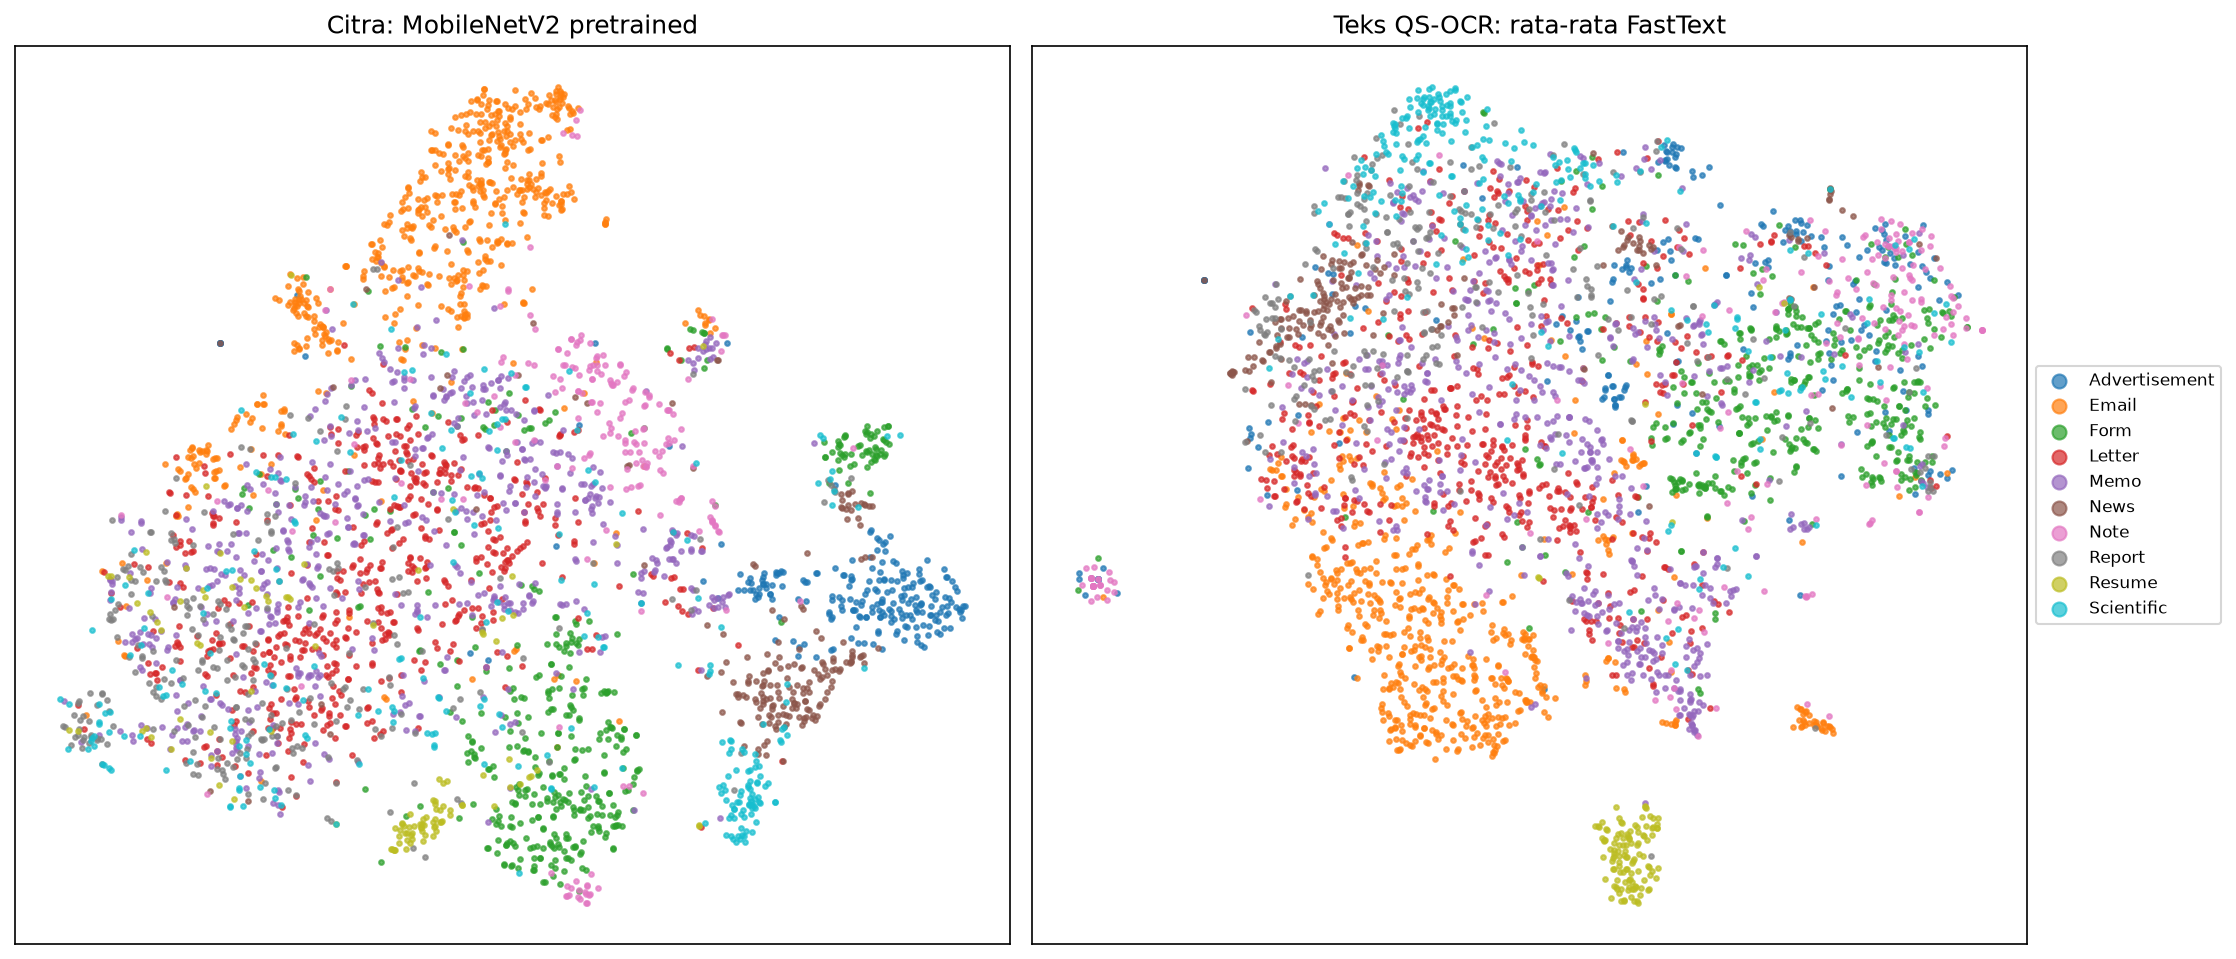
\includegraphics[width=\textwidth]{../../reports/figures/fase2_eda_tsne.png}
  \caption{Proyeksi t-SNE fitur citra (kiri, MobileNetV2 ImageNet) dan fitur teks
  (kanan, rata-rata FastText QS-OCR), diwarnai menurut kelas}
  \label{fig:eda-tsne}
\end{figure}

\subsubsection{Komplementaritas dan Kurasi}

F1 \textit{probe} per kelas memperlihatkan di mana tiap modalitas unggul
(Tabel~\ref{tab:eda-komplementer}).

\begin{table}[H]
  \centering
  \caption{F1 \textit{probe} per kelas: citra vs teks QS-OCR}
  \label{tab:eda-komplementer}
  \fontsize{10}{12}\selectfont
  \begin{tabular}{|l|c|c|c|}
    \hline
    \textbf{Kelas} & \textbf{Citra} & \textbf{Teks} & \textbf{Teks $-$ citra} \\ \hline
    Resume & 0,710 & 0,947 & $+0{,}237$ \\ \hline
    Scientific & 0,446 & 0,523 & $+0{,}077$ \\ \hline
    Email & 0,899 & 0,918 & $+0{,}019$ \\ \hline
    Memo & 0,674 & 0,627 & $-0{,}047$ \\ \hline
    Report & 0,421 & 0,366 & $-0{,}055$ \\ \hline
    News & 0,837 & 0,764 & $-0{,}073$ \\ \hline
    Form & 0,813 & 0,737 & $-0{,}076$ \\ \hline
    Letter & 0,727 & 0,624 & $-0{,}103$ \\ \hline
    Note & 0,686 & 0,397 & $-0{,}289$ \\ \hline
    Advertisement & 0,886 & 0,589 & $-0{,}297$ \\ \hline
  \end{tabular}
\end{table}

Teks unggul pada Resume, Scientific, dan Email; citra unggul jauh pada Advertisement dan
Note, tepat kelas yang teksnya paling sering kosong atau rusak. Komplementaritas ini sudah
terlihat sebelum pelatihan apa pun, dan menjadi dasar harapan bahwa fusion menolong.
Kurasi menemukan 101 dokumen Note dan 62 Advertisement yang teksnya bermasalah tetapi
citranya baik: di situlah fusion seharusnya paling berguna.

Kurasi \textbf{menandai, tidak membuang}, karena derau OCR adalah objek penelitian.
Selain penanda teks, ditemukan 12 pasangan duplikat (korelasi \textit{thumbnail} tinggi
dan dikonfirmasi kemiripan teks), dengan 1, 5, dan 4 pasangan yang terbelah antara data
latih dan uji pada seed 42, 43, dan 44. Jumlah ini terlalu kecil untuk memengaruhi
akurasi atas 2.682 dokumen uji secara berarti. Jalan pintas kode ID arsip
\parencite{larson2025} juga diuji: classifier yang hanya diberi tiga digit awal kode ID
dalam teks OCR mencapai OA 0,2782, sepuluh poin di atas kelas mayoritas tetapi jauh di
bawah \textit{probe} teks.

Probe yang sama pada keempat kondisi OCR menghasilkan PaddleOCR 0,6864, QS-OCR 0,6685,
EasyOCR 0,6521, dan Tesseract 0,6499. Urutan ini nantinya cocok dengan urutan akurasi
cabang teks yang dilatih (Subbagian~\ref{sec:hasil-teks}).

\subsection{Kualitas Keluaran OCR}\label{sec:hasil-ocr}

Proksi kualitas setiap kondisi disajikan pada Tabel~\ref{tab:proksi}.

\begin{table}[H]
  \centering
  \caption{Proksi kualitas OCR per kondisi (seluruh 3.482 halaman)}
  \label{tab:proksi}
  \fontsize{10}{12}\selectfont
  \begin{tabular}{|l|r|r|r|r|r|}
    \hline
    \textbf{Kondisi} & \textbf{\makecell{Kata/halaman\\(median)}} &
    \textbf{\makecell{Halaman\\kosong}} & \textbf{\makecell{OOV\\median}} &
    \textbf{\makecell{OOV\\rata-rata}} & \textbf{\makecell{Jaccard\\ke QS-OCR}} \\ \hline
    QS-OCR & 160 & 1,06\% & 0,055 & 0,098 & 1 \\ \hline
    Tesseract & 161 & 0,60\% & 0,057 & 0,115 & 0,920 \\ \hline
    EasyOCR & 157 & 0,17\% & 0,136 & 0,232 & 0,693 \\ \hline
    PaddleOCR & 162 & 0,06\% & 0,054 & 0,124 & 0,864 \\ \hline
  \end{tabular}
\end{table}

PaddleOCR menghasilkan teks paling lengkap: halaman kosongnya hampir nol dan OOV
mediannya terendah, walaupun dibaca dari JPG. EasyOCR menonjol ke arah sebaliknya, dengan
OOV median 2,5 kali mesin lain dan kesepakatan terendah dengan semua mesin (Jaccard 0,69
sampai 0,73). Tesseract-JPG paling dekat dengan QS-OCR, wajar karena mesinnya sekeluarga.
Untuk semua mesin, kelas dengan OOV tertinggi adalah Note (median 0,25 sampai 0,64),
disusul Advertisement dan News.

Biayanya sangat berbeda: EasyOCR di GPU 4~GB sekitar 22 kali lebih lambat daripada
Tesseract di CPU (Tabel~\ref{tab:waktu}).

\subsection{Pengaruh Mesin OCR terhadap Cabang Teks (RM1)}\label{sec:hasil-teks}

Akurasi cabang teks per kondisi disajikan pada Tabel~\ref{tab:teks}, dan uji
McNemar-nya pada Tabel~\ref{tab:mcnemar-ocr}.

\begin{table}[H]
  \centering
  \caption{Akurasi cabang teks (FastText + CNN~1D) per kondisi OCR}
  \label{tab:teks}
  \fontsize{10}{12}\selectfont
  \begin{tabular}{|l|c|c|c|}
    \hline
    \textbf{Kondisi} & \textbf{OA} & \textbf{Macro F1} & \textbf{OA per seed (42/43/44)} \\ \hline
    QS-OCR & $0{,}7266 \pm 0{,}0059$ & $0{,}7017 \pm 0{,}0053$ & 0,7345 / 0,7248 / 0,7204 \\ \hline
    Tesseract & $0{,}6970 \pm 0{,}0047$ & $0{,}6547 \pm 0{,}0083$ & 0,6913 / 0,7028 / 0,6969 \\ \hline
    EasyOCR & $0{,}7155 \pm 0{,}0061$ & $0{,}6862 \pm 0{,}0095$ & 0,7155 / 0,7081 / 0,7230 \\ \hline
    PaddleOCR & $\mathbf{0{,}7514 \pm 0{,}0043}$ & $\mathbf{0{,}7200 \pm 0{,}0057}$ &
    0,7498 / 0,7573 / 0,7472 \\ \hline
  \end{tabular}
\end{table}

\begin{table}[H]
  \centering
  \caption{McNemar antar-kondisi OCR untuk cabang teks (Holm per seed, $\alpha = 0{,}05$)}
  \label{tab:mcnemar-ocr}
  \fontsize{10}{12}\selectfont
  \begin{tabular}{|l|c|c|}
    \hline
    \textbf{Pasangan (a $-$ b)} & \textbf{Selisih OA rerata} & \textbf{Seed signifikan} \\ \hline
    Tesseract $-$ PaddleOCR & $-0{,}0544$ & 3/3 \\ \hline
    EasyOCR $-$ PaddleOCR & $-0{,}0359$ & 3/3 \\ \hline
    QS-OCR $-$ Tesseract & $+0{,}0296$ & 3/3 \\ \hline
    QS-OCR $-$ PaddleOCR & $-0{,}0249$ & 2/3 \\ \hline
    Tesseract $-$ EasyOCR & $-0{,}0185$ & 2/3 \\ \hline
    QS-OCR $-$ EasyOCR & $+0{,}0111$ & 0/3 \\ \hline
  \end{tabular}
\end{table}

\textbf{H1 didukung.} Dengan embedding, arsitektur, pembagian data, dan hiperparameter
dikunci, mesin OCR saja menggeser OA cabang teks sebesar \textbf{5,4 poin}, dari 0,6970
(Tesseract-JPG) ke 0,7514 (PaddleOCR). Tiga pasangan berbeda nyata di ketiga seed. Selisih
terbesar sekitar 11 kali simpangan baku antar-seed cabang teks. Dugaan arah juga benar:
QS-OCR mengungguli Tesseract-JPG di ketiga seed.

Tiga pengamatan menyertai hasil ini.

\textbf{Mesin lebih menentukan daripada sumber citra.} PaddleOCR yang membaca JPG
mengalahkan QS-OCR yang dibaca dari TIF asli (+2,5 poin, nyata di dua seed), sedangkan
Tesseract pada JPG kalah dari QS-OCR ($-3{,}0$ poin, nyata di tiga seed). Teks QS-OCR yang
selama ini dipakai sebagai acuan karena itu bukan batas atas.

\textbf{Proksi OOV tidak meramalkan kegunaan teks.} EasyOCR memiliki OOV terburuk dan
kesepakatan terendah, tetapi cabang teksnya lebih akurat daripada Tesseract-JPG.
Sebaliknya, \textit{linear probe} tanpa pelatihan pada rata-rata vektor FastText
meramalkan urutan mesin dengan cukup baik: PaddleOCR 0,686 $>$ QS-OCR 0,669 $>$ EasyOCR
0,652 $\approx$ Tesseract 0,650. Untuk memilih mesin OCR bagi tugas klasifikasi, probe
kecil lebih berguna daripada statistik OOV.

\textbf{Tidak ada mesin yang terbaik di semua kelas.} Keunggulan PaddleOCR tersebar di
kelas yang kaya teks: terhadap QS-OCR, F1 Advertisement naik 8,5 poin, Letter 7,4,
Report 5,1, dan Memo 4,5. Namun F1 Note \emph{turun} 9,2 poin (0,621 ke 0,529). Note
adalah kelas dengan OOV tertinggi untuk semua mesin, dan 48,3\% halamannya berisi kurang
dari 20 kata.

\subsection{Fusion per Kondisi OCR (RM3)}\label{sec:hasil-fusion}

Hasil utama disajikan pada Tabel~\ref{tab:utama} dan Gambar~\ref{fig:grid}.

\begin{table}[H]
  \centering
  \caption{OA rerata $\pm$ simpangan baku antar-seed per kondisi OCR}
  \label{tab:utama}
  \fontsize{9}{11}\selectfont
  \setlength{\tabcolsep}{3.5pt}
  \begin{tabular}{|l|c|c|c|c|c|}
    \hline
    \textbf{Kondisi} & \textbf{IMAGE} & \textbf{TEXT} & \textbf{LATE} & \textbf{CONCAT} &
    \textbf{ORACLE} \\ \hline
    QS-OCR & $0{,}8169 \pm 0{,}0257$ & $0{,}7266 \pm 0{,}0059$ & $0{,}8456 \pm 0{,}0221$ &
    $0{,}8316 \pm 0{,}0119$ & $0{,}9023 \pm 0{,}0127$ \\ \hline
    Tesseract & $0{,}8169 \pm 0{,}0257$ & $0{,}6970 \pm 0{,}0047$ & $0{,}8376 \pm 0{,}0174$ &
    $0{,}8349 \pm 0{,}0102$ & $0{,}8950 \pm 0{,}0086$ \\ \hline
    EasyOCR & $0{,}8169 \pm 0{,}0257$ & $0{,}7155 \pm 0{,}0061$ & $0{,}8538 \pm 0{,}0158$ &
    $0{,}8567 \pm 0{,}0034$ & $0{,}8972 \pm 0{,}0091$ \\ \hline
    PaddleOCR & $0{,}8169 \pm 0{,}0257$ & $0{,}7514 \pm 0{,}0043$ &
    $\mathbf{0{,}8653 \pm 0{,}0122}$ & $\mathbf{0{,}8674 \pm 0{,}0014}$ &
    $0{,}9079 \pm 0{,}0105$ \\ \hline
  \end{tabular}
\end{table}

\begin{figure}[H]
  \centering
  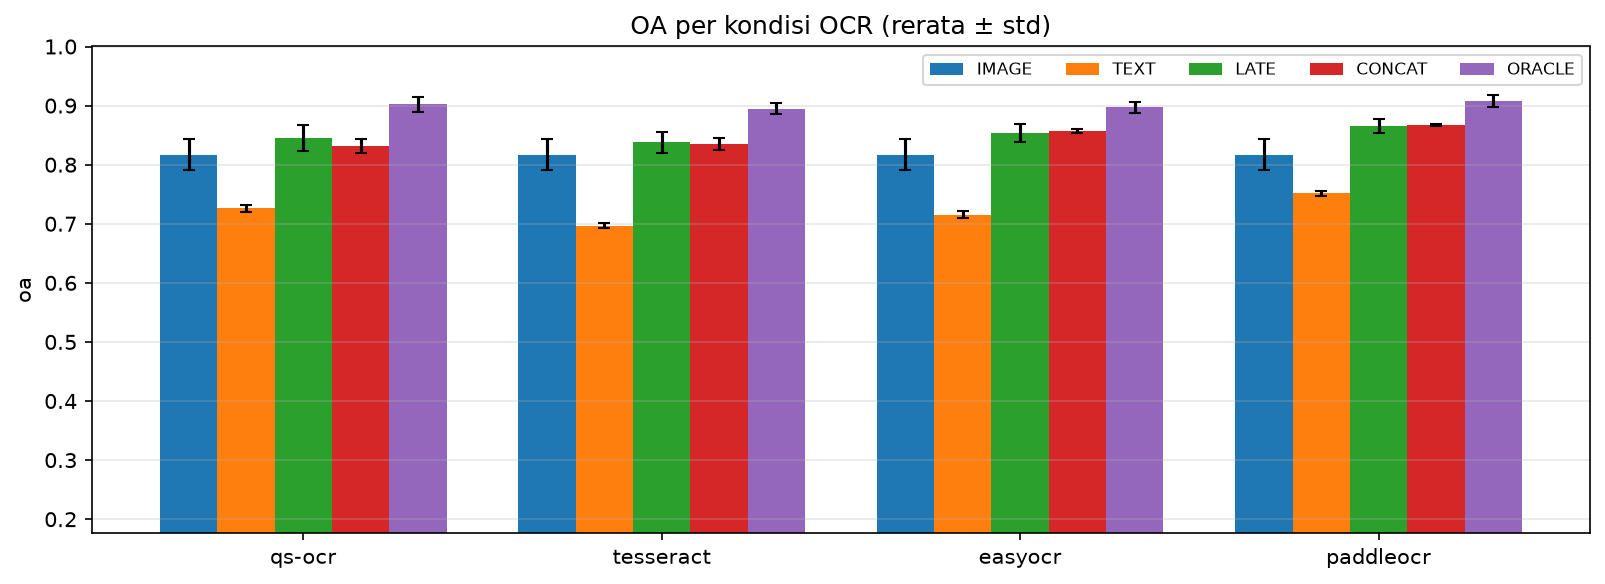
\includegraphics[width=\textwidth]{../../reports/figures/fase2_grid_oa.png}
  \caption{OA per kondisi OCR, rerata $\pm$ simpangan baku tiga seed}
  \label{fig:grid}
\end{figure}

\textbf{OCR yang lebih baik menaikkan fusion, untuk kedua aturan.} Dari Tesseract-JPG ke
PaddleOCR, LATE naik 2,8 poin dan CONCAT 3,2 poin, berbeda nyata di ketiga seed. Sel
terbaik adalah \textbf{CONCAT dengan PaddleOCR, $0{,}8674 \pm 0{,}0014$} (macro F1
$0{,}8524 \pm 0{,}0016$), 3,3 poin di atas fusion \textit{end-to-end} Fase~1 (0,8342).
Macro F1 mengikuti pola yang sama dengan OA.

Seberapa banyak potensi teks dipanen fusion (Persamaan~\ref{eq:panen}) disajikan pada
Tabel~\ref{tab:panen}. Sebagai pembanding, fusion \textcite{audebert2020} memanen 43\%
potensinya, dan fusion \textit{end-to-end} Fase~1 29\%.

\begin{table}[H]
  \centering
  \caption{Potensi oracle dan bagian yang dipanen fusion (rerata seed)}
  \label{tab:panen}
  \fontsize{10}{12}\selectfont
  \begin{tabular}{|l|c|c|c|c|c|}
    \hline
    \textbf{Kondisi} & \textbf{Potensi} & \textbf{LATE $-$ IMAGE} & \textbf{Panen LATE} &
    \textbf{CONCAT $-$ IMAGE} & \textbf{Panen CONCAT} \\ \hline
    QS-OCR & 0,0854 & $+0{,}0287$ & 34\% & $+0{,}0147$ & 13\% \\ \hline
    Tesseract & 0,0781 & $+0{,}0206$ & 25\% & $+0{,}0180$ & 19\% \\ \hline
    EasyOCR & 0,0803 & $+0{,}0369$ & 46\% & $+0{,}0398$ & 46\% \\ \hline
    PaddleOCR & 0,0910 & $+0{,}0483$ & 52\% & $+0{,}0505$ & 52\% \\ \hline
  \end{tabular}
\end{table}

LATE berada di atas IMAGE di 12 dari 12 sel (minimum $+0{,}006$). CONCAT tidak: pada
QS-OCR seed 43, CONCAT 0,8188 berada di bawah IMAGE 0,8386.

\textbf{H3a didukung untuk LATE, lemah untuk CONCAT.} Korelasi Spearman antara OA cabang
teks dan $\Delta_\text{teks}$ LATE adalah 0,683 atas 12 sel; terhadap kenaikan LATE di
atas IMAGE 0,517, dan terhadap panen LATE 0,65. Untuk CONCAT, $\Delta_\text{teks}$ dengan
pengganti kosong tidak sah sebagai ukuran (Subbagian~\ref{sec:hasil-missing}), sehingga
yang dipakai adalah kenaikan di atas IMAGE; korelasinya hanya 0,287. Akurasi teks juga
bukan satu-satunya penentu: cabang teks EasyOCR lebih lemah daripada QS-OCR, tetapi
dipanen jauh lebih banyak (46\% vs 34\% untuk LATE, 46\% vs 13\% untuk CONCAT).

\textbf{H3b tidak didukung; arahnya justru terbalik bila cabang citra lemah.} Hasil
McNemar LATE vs CONCAT disajikan pada Tabel~\ref{tab:late-concat}.

\begin{table}[H]
  \centering
  \caption{McNemar LATE vs CONCAT per kondisi (Holm per seed); \enquote{--} berarti tidak
  berbeda nyata}
  \label{tab:late-concat}
  \fontsize{10}{12}\selectfont
  \begin{tabular}{|c|c|c|c|c|c|}
    \hline
    \textbf{Seed} & \textbf{IMAGE} & \textbf{QS-OCR} & \textbf{Tesseract} & \textbf{EasyOCR} &
    \textbf{PaddleOCR} \\ \hline
    42 & 0,8315 & LATE lebih baik & -- & -- & -- \\ \hline
    43 & 0,8386 & LATE lebih baik & -- & -- & LATE lebih baik \\ \hline
    44 & 0,7808 & CONCAT lebih baik & -- & CONCAT lebih baik & CONCAT lebih baik \\ \hline
  \end{tabular}
\end{table}

Rerata kedua aturan hampir sama (selisih paling besar 1,4 poin), dan pemenangnya
bergantung pada kekuatan cabang citra. LATE unggul nyata saat cabang citra kuat (seed 42
dan 43), sedangkan CONCAT unggul nyata di tiga dari empat kondisi saat cabang citra lemah
(seed 44). Rata-rata tanpa bobot ikut jatuh bersama cabang yang lemah, sedangkan
\textit{head} yang dilatih menyesuaikan bobotnya. CONCAT juga jauh lebih stabil
antar-seed (simpangan baku 0,0014 sampai 0,0119, LATE 0,0122 sampai 0,0221). Untuk cabang
\emph{teks} yang lemah (Tesseract-JPG), kedua aturan tidak berbeda nyata di seed mana pun.

Matriks konfusi sel terbaik ditunjukkan Gambar~\ref{fig:konfusi}. Kelas tersulit tetap
Scientific (\textit{recall} 0,46), yang terutama tertukar dengan Report dan Form, sama
dengan pola pada ketiga paper rujukan.

\begin{figure}[H]
  \centering
  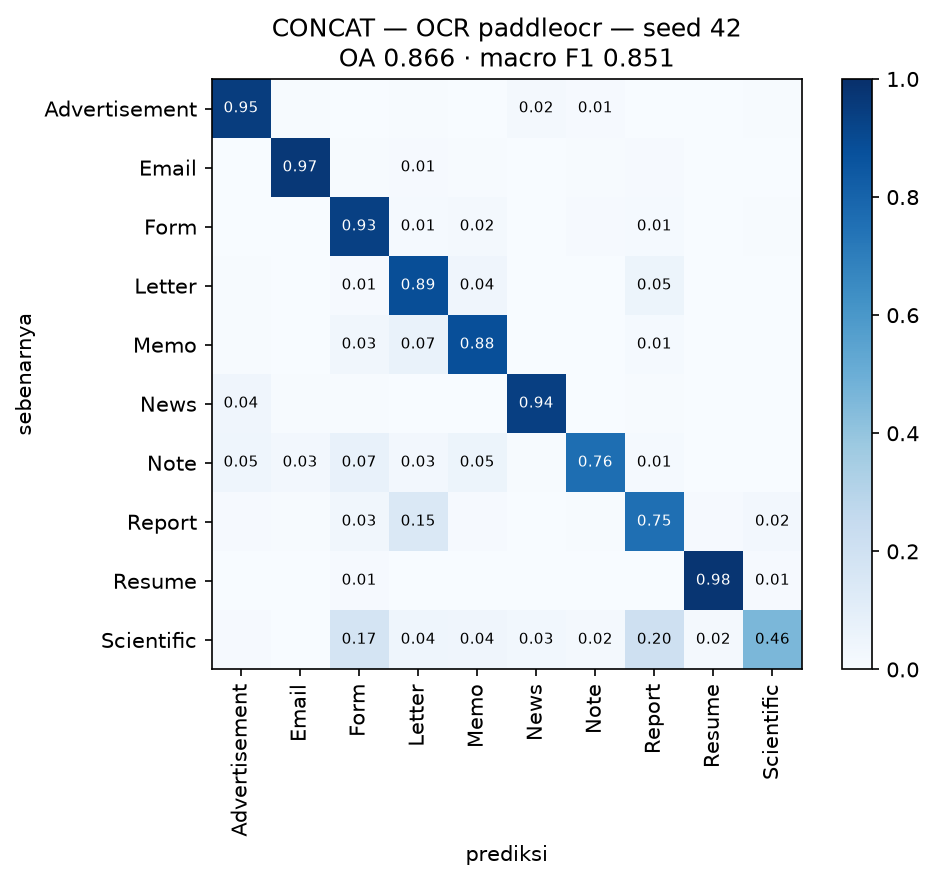
\includegraphics[width=0.72\textwidth]{../../reports/figures/fase2_konfusi_terbaik.png}
  \caption{Matriks konfusi ternormalisasi per baris, CONCAT dengan PaddleOCR, seed 42}
  \label{fig:konfusi}
\end{figure}

\subsection{Uji \textit{Missing Modality}}\label{sec:hasil-missing}

\subsubsection{Pengganti kosong: anomali}

Hasil uji dengan pengganti kosong, yang dirancang sebelum eksekusi, disajikan pada
Tabel~\ref{tab:missing-kosong}.

\begin{table}[H]
  \centering
  \caption{Uji \textit{missing modality} dengan pengganti kosong: selisih OA terhadap model
  unimodal modalitas yang tersisa (rerata seed)}
  \label{tab:missing-kosong}
  \fontsize{10}{12}\selectfont
  \begin{tabular}{|l|c|c|c|c|}
    \hline
    \textbf{Kondisi} & \textbf{\makecell{LATE tanpa teks\\$-$ IMAGE}} &
    \textbf{\makecell{CONCAT tanpa teks\\$-$ IMAGE}} &
    \textbf{\makecell{LATE tanpa citra\\$-$ TEXT}} &
    \textbf{\makecell{CONCAT tanpa citra\\$-$ TEXT}} \\ \hline
    QS-OCR & $-0{,}022$ & $-0{,}563$ & $-0{,}268$ & $-0{,}112$ \\ \hline
    Tesseract & $-0{,}008$ & $-0{,}591$ & $-0{,}271$ & $-0{,}135$ \\ \hline
    EasyOCR & $-0{,}001$ & $-0{,}137$ & $-0{,}337$ & $-0{,}202$ \\ \hline
    PaddleOCR & $-0{,}003$ & $-0{,}301$ & $-0{,}349$ & $-0{,}216$ \\ \hline
  \end{tabular}
\end{table}

Hanya LATE tanpa teks yang berperilaku seperti seharusnya: ia mendarat di IMAGE (selisih
paling besar 2,2 poin). CONCAT tanpa teks jatuh \textbf{jauh di bawah cabang citra
sendiri}, sampai 59 poin, dan semua versi tanpa citra jatuh di bawah cabang teks sendiri.
Kehilangan satu modalitas tidak mungkin lebih buruk daripada model unimodal modalitas yang
tersisa, kecuali penggantinya keluar distribusi bagi model. Dugaan awal kami untuk CONCAT
adalah bahwa \textit{head} belajar \enquote{teks kosong $\Rightarrow$ Note}, karena
sebagian halaman Note pada QS-OCR kosong. Dua dugaan ini diuji pada uji lanjutan (H4a dan
H4b).

\subsubsection{Uji lanjutan: pengganti rerata dan \textit{head} tanpa teks kosong}

Dokumen yang kosong menurut model berjumlah 27 (QS-OCR: 20 Note, 7 Advertisement), 11
(Tesseract: 6 Note, 5 Advertisement), dan 0 untuk EasyOCR maupun PaddleOCR. Di bagian latih
\textit{head} terdapat 4 sampai 8 dokumen kosong untuk QS-OCR dan 2 sampai 4 untuk
Tesseract, dari 720 dokumen. Hasil uji lanjutan disajikan pada Tabel~\ref{tab:missing-lanjutan}.

\begin{table}[H]
  \centering
  \caption{Uji lanjutan: selisih OA terhadap model unimodal modalitas yang tersisa (rerata
  seed)}
  \label{tab:missing-lanjutan}
  \fontsize{10}{12}\selectfont
  \begin{tabularx}{\textwidth}{|>{\raggedright\arraybackslash}X|c|c|c|c|}
    \hline
    \textbf{Selisih} & \textbf{QS-OCR} & \textbf{Tesseract} & \textbf{EasyOCR} &
    \textbf{PaddleOCR} \\ \hline
    CONCAT tanpa teks, kosong $-$ IMAGE & $-0{,}563$ & $-0{,}591$ & $-0{,}137$ & $-0{,}301$ \\ \hline
    CONCAT tanpa teks, rerata $-$ IMAGE & $-0{,}108$ & $-0{,}130$ & $-0{,}026$ & $-0{,}027$ \\ \hline
    CONCAT\_nonkosong tanpa teks, kosong $-$ IMAGE & $-0{,}496$ & $-0{,}633$ & $-0{,}137$ & $-0{,}301$ \\ \hline
    LATE tanpa teks, rerata $-$ IMAGE & $-0{,}132$ & $-0{,}129$ & $-0{,}076$ & $-0{,}074$ \\ \hline
    LATE tanpa citra, rerata $-$ TEXT & $-0{,}029$ & $-0{,}036$ & $-0{,}040$ & $-0{,}042$ \\ \hline
    CONCAT tanpa citra, rerata $-$ TEXT & $-0{,}005$ & $+0{,}006$ & $-0{,}017$ & $-0{,}014$ \\ \hline
    CONCAT\_nonkosong $-$ CONCAT (masukan lengkap) & $+0{,}006$ & $+0{,}003$ & 0 & 0 \\ \hline
  \end{tabularx}
\end{table}

\textbf{H4a didukung sebagian.} Dengan pengganti rerata, kedua aturan tanpa citra
mendarat paling jauh 4,2 poin di bawah cabang teks, padahal dengan pengganti kosong 11
sampai 35 poin. Kejatuhan tanpa citra karena itu artefak pengganti. CONCAT tanpa teks pulih
sebagian besar (QS-OCR $-0{,}563 \rightarrow -0{,}108$; Tesseract
$-0{,}591 \rightarrow -0{,}130$) dan mendarat dekat IMAGE pada EasyOCR dan PaddleOCR
($-0{,}026$ dan $-0{,}027$). Pada QS-OCR dan Tesseract masih tersisa 11 sampai 13 poin di
bawah IMAGE, dengan sebaran besar antar-seed ($-0{,}03$ sampai $-0{,}20$). Pada kedua
kondisi itu, \textit{head} memang tidak dapat bekerja setara cabang citra tanpa teks.

\textbf{H4b tidak didukung.} Prasyaratnya terpenuhi: membuang dokumen kosong hanya
menggeser CONCAT dengan masukan lengkap 0,3 sampai 0,6 poin. Kriteria (i) juga terpenuhi:
dengan teks kosong, porsi prediksi Note membengkak dari 0,058 (porsi sebenarnya) menjadi
0,727, 0,756, 0,192, dan 0,320 (QS-OCR, Tesseract, EasyOCR, PaddleOCR). Namun kriteria (ii)
gagal di keempat kondisi. \textit{Head} tanpa dokumen kosong tetap menarik prediksi ke Note
(0,483 pada QS-OCR, bahkan naik ke 0,817 pada Tesseract). Bukti paling langsung datang
dari EasyOCR dan PaddleOCR: tidak ada satu pun dokumen kosong pada kedua kondisi itu, tetapi
tarikan ke Note tetap muncul. Dengan pengganti rerata, porsi Note kembali normal (0,04
sampai 0,09 per sel). Tarikan itu karena itu milik vektor teks kosong, bukan hasil belajar
dari dokumen kosong di data latih. Dugaan yang tersisa, dan belum diuji, adalah bahwa Note
sebagai kelas berteks terpendek memiliki fitur yang paling dekat dengan fitur teks kosong,
sehingga \textit{head} berekstrapolasi ke arah Note. Besar tarikannya berubah tajam
antar-seed (PaddleOCR: 0,044 / 0,532 / 0,383), sesuai dengan ekstrapolasi di luar
distribusi.

\textbf{Pengganti rerata tidak netral untuk LATE.} LATE tanpa teks dengan pengganti kosong
mendarat di IMAGE, tetapi dengan rerata logit latih ia jatuh 7 sampai 13 poin di bawah
IMAGE (negatif di setiap sel). Rerata logit menambahkan bias kelas tetap ke logit citra,
dan logit latih cabang teks berasal dari model yang dilatih pada dokumen itu sendiri.
Jadi, pengganti yang sah berbeda menurut aturan: pengganti kosong untuk LATE tanpa teks,
pengganti rerata untuk CONCAT tanpa teks dan untuk semua versi tanpa citra.

\subsection{Posisi terhadap Literatur}\label{sec:posisi-hasil}

Tabel~\ref{tab:literatur} menempatkan hasil ini di samping studi rujukan.

\begin{table}[H]
  \centering
  \caption{OA fusion pada Tobacco3482 dan protokolnya}
  \label{tab:literatur}
  \fontsize{10}{12}\selectfont
  \begin{tabularx}{\textwidth}{|>{\raggedright\arraybackslash}X|>{\raggedright\arraybackslash}p{6.2cm}|c|}
    \hline
    \textbf{Studi} & \textbf{Protokol} & \textbf{OA fusion} \\ \hline
    \textcite{kashyap2026} & dilatih pada RVL-CDIP, Tobacco3482 hanya diuji & 0,9200 \\ \hline
    \textcite{audebert2020} & 800 dokumen latih, tiga run & 0,878 \\ \hline
    Fase~1 (replikasi Audebert) & 800 dokumen latih, tiga seed & $0{,}8342 \pm 0{,}0105$ \\ \hline
    \textbf{Penelitian ini, CONCAT + PaddleOCR} & 800 dokumen latih, tiga seed &
    $\mathbf{0{,}8674 \pm 0{,}0014}$ \\ \hline
  \end{tabularx}
\end{table}

Angka antarbaris tidak sepenuhnya sebanding. \textcite{kashyap2026} melatih pada
$\pm$320.000 dokumen RVL-CDIP, dan angka Tobacco3482-nya tidak konsisten dengan
protokolnya sendiri (Subbagian~\ref{sec:kajian-pustaka}). Yang sebanding langsung adalah
dua baris terakhir: dengan data dan pembagian yang sama, mengganti mesin OCR dan aturan
fusion menaikkan fusion 3,3 poin dan memperkecil simpangan baku antar-seed tujuh kali lipat.
